%        File: definitions.tex
%     Created: Wed Sep 09 11:00 PM 2020 M
% Last Change: Wed Sep 09 11:00 PM 2020 M
%

\documentclass[a4paper]{article}
\usepackage{amsmath}%
\usepackage{amsfonts}%
\usepackage{amssymb}%
\usepackage{graphicx}
\usepackage{enumitem}
%-------------------------------------------
\newtheorem{theorem}{Theorem}
\newtheorem{acknowledgement}[theorem]{Acknowledgement}
\newtheorem{algorithm}[theorem]{Algorithm}
\newtheorem{axiom}[theorem]{Axiom}
\newtheorem{case}[theorem]{Case}
\newtheorem{claim}[theorem]{Claim}
\newtheorem{conclusion}[theorem]{Conclusion}
\newtheorem{condition}[theorem]{Condition}
\newtheorem{conjecture}[theorem]{Conjecture}
\newtheorem{corollary}[theorem]{Corollary}
\newtheorem{criterion}[theorem]{Criterion}
\newtheorem{definition}[theorem]{Definition}
\newtheorem{example}[theorem]{Example}
\newtheorem{exercise}[theorem]{Exercise}
\newtheorem{lemma}[theorem]{Lemma}
\newtheorem{notation}[theorem]{Notation}
\newtheorem{problem}[theorem]{Problem}
\newtheorem{proposition}[theorem]{Proposition}
\newtheorem{remark}[theorem]{Remark}
\newtheorem{solution}[theorem]{Solution}
\newtheorem{summary}[theorem]{Summary}
\newenvironment{proof}[1][Proof]{\textbf{#1.} }{\ \rule{0.5em}{0.5em}}
\setlength{\textwidth}{7.0in}
\setlength{\oddsidemargin}{-0.35in}
\setlength{\topmargin}{-0.5in}
\setlength{\textheight}{9.0in}
\setlength{\parindent}{0.3in}

\newcommand{\N}{\mathbb{N}}
\newcommand{\Z}{\mathbb{Z}}
\newcommand{\Q}{\mathbb{Q}}
\newcommand{\R}{\mathbb{R}}
\newcommand{\U}{\mathbb{U}}
\graphicspath { {.} }


\usepackage{listings}
\usepackage{color}

\definecolor{dkgreen}{rgb}{0,0.6,0}
\definecolor{gray}{rgb}{0.5,0.5,0.5}
\definecolor{mauve}{rgb}{0.58,0,0.82}

\lstset{frame=tb,
    language=Java,aboveskip=3mm,belowskip=3mm,showstringspaces=false,columns=flexible,basicstyle={\small\ttfamily},numbers=none,numberstyle=\tiny\color{gray},keywordstyle=\color{blue},commentstyle=\color{dkgreen},stringstyle=\color{mauve},breaklines=true,breakatwhitespace=true,tabsize=3
  }

\begin{document}
\title{Discrete Structures Definitions}
\author{Levi Shafter}
\maketitle
\pagebreak

\section{Vocabulary}

\subsection{Logic}
\paragraph{logic} The study of formal reasoning
\paragraph{proposition} A statement that is either true or false
\paragraph{truth value} A proposition's truth value is a value indicating whether the proposition is actually true or false
\paragraph{compound proposition} A proposition created by connecting individual propositions with logical operations
\paragraph{logical operation} Combines propositions using a particular composition rule
\paragraph{conjunction} When two propositions are combined with a logical ``and'' operator. ex: $p \land q$
\paragraph{disjunction} When two propositions are combined with a logical ``or'' operator. 
\paragraph{truth table} shows the truth value of a compound proposition for every possible combination of truth values for the variables contained in the compound proposition
\paragraph{exclusive or} p and q evaluates to true when p is true and q is false or when q is true and p is false in the compound proposition $p \oplus q$
\paragraph{inclusive or} evaluates to true when one or both of the propositions are true. ex: $p \lor q$
\paragraph{negation} acts on just one proposition and has the effect of reversing the truth value of the proposition. ex: $\lnot p$
\paragraph{conditional operation} The proposition p → q is read "if p then q". The proposition p → q is false if p is true and q is false; otherwise, p → q is true. 
\paragraph{conditional proposition} A compound proposition that uses a conditional operation
\paragraph{conditional statement} A conditional proposition expressed in English
\paragraph{argument} A sequence of propositions. It is \textbf{valid} if the conclusion is true whenever the hypotheses are all true, otherwise the argument is \textbf{invalid}
\paragraph{hypothesis} One of the propositions before the conclusion of the argument
\paragraph{conclusion} The final proposition in an argument
\paragraph{converse} The converse of $p \implies q$ is $q \implies p$
\paragraph{contrapositive} The contrapositive of $p \implies q$ is $\lnot q \implies \lnot p$
\paragraph{inverse} The inverse of $p \implies q$ is $\lnot p \implies \lnot q$
\paragraph{biconditional operation} If p and q are propositions, the proposition "p if and only if q" is expressed with the biconditional operation and is denoted $p \iff q$. The proposition $p \iff q$ is true when p and q have the same truth value and is false when p and q have different truth values. This can also be notated as ``iff''
\paragraph{tautology} A compound proposition that is always true regardless of any truth values of the propositions within it
\paragraph{contradiction} A compound proposition that is always false regardless of any truth values of the propositions within it
\paragraph{logical equivalence} When two compound propositions have the same truth value regardless of the truth values of their individual propositions
\paragraph{logical order of operations} The order of operations when it comes to logical operations in order of priority from left to right is as follows: $()$, $\lnot$, $\land$, $\lor$
\paragraph{predicate} A logical statement whose truth value is a function of one or more variables
\paragraph{domain} The set of all possible values for a variable in a predicate
\paragraph{universal quantifier} The symbol $\forall$ which translates to ``for all''
\paragraph{universally quantified statement} A statement using a universal quantifier. Ex: $\forall x P(x)$ reads ``for all x, P(x)''
\paragraph{counterexample} A counterexample for a universally quantified statement is an element in the domain for which the predicate is false.
\paragraph{existential quantifier} The symbol $\exists$ which translates to ``there exists''
\paragraph{existentially quantified statement} A statement using an existential quantifier. Ex: $\exists x P(x)$ reads ``there exists an x, such that P(x)''
\paragraph{free variable} A variable in a predicate which is free to take on any value in the domain without making the statement false
\paragraph{bound variable} A variable bound to a quantifier so that it is restricted to certain values without making the statement false
\paragraph{nested quantifiers} Quantifiers within a logical expression that contains multiple quantifiers that bind different variables in the same predicate
\paragraph{logical proof} A sequence of steps, each of which consists of a proposition and a justification
\paragraph{element} A value that can be plugged in for a variable is called an element of the domain of that variable
\paragraph{arbitrary (element of a domain)} Has no special properties other than those shared by all the elements of the domain
\paragraph{particular (element of a domain)} May have properties that are not shared by all the elements of the domain
\paragraph{existential/universal instantiation} These rules replace a quantified variable with an element of the domain
\paragraph{existential/universal generalization} These rules replace an element of the domain with a quantified variable
\pagebreak
\subsection{Proofs}
\paragraph{even number} An integer $x$ is even if there is an integer $k$ such that $x = 2k$.
\paragraph{odd number} An integer $x$ is odd if there is an integer $k$ such that $x = 2k+1$.
\paragraph{parity} Whether a number is odd or even.
\paragraph{rational number} A number r is rational if there exist integers $x$ and $y$ such that $y \neq 0$ and $r = x/y$.
\paragraph{divides} An integer $x$ divides an integer $y$ if and only if $x \neq 0$ and $y = kx$, for some integer $k$. The fact that $x$ divides $y$ is denoted $x|y$. If $x$ does not divide $y$, then that fact is denoted $x \nmid y$. If $x$ divides $y$, then $y$ is said to be a \textbf{multiple} of $x$, and $x$ is a \textbf{factor} or \textbf{divisor} of $y$.
\paragraph{prime number} an integer $n$ is prime if and only if $n > 1$, and for every positive integer $M$, if $m|n$, then $m = 1$ or $m = n$.
\paragraph{composite number} An integer $n$ is composite if and only if $n > 1$, and there is an integer $m$ such that $1 < m < n$ and $m|n$.
\paragraph{positive/negative number} A real number $x$ is \textbf{positive} if and only if $x > 0$. A real number $x$ is \textbf{negative} if and only if $x < 0$. A real number $x$ is \textbf{non-negative} if and only if $x \geq 0$. A real number $x$ is \textbf{non-positive} if and only if $x \leq 0$.
\paragraph{theorem} A statement that can be proven to be true
\paragraph{proof} Consists of a series of steps, each of which follows logically from assumptions, or from previously proven statements, whose final step should result in the statement of the theorem being proven
\paragraph{axiom} A statement assumed to be true
\paragraph{perfect square} A number $n$ is a perfect square if $n = k^2$ for some integer $k$.
\paragraph{proof by exhaustion} A proof that checks each element of a statement individually
\paragraph{universal generalization} A method to prove a universal statement by naming an arbitrary object in the domain and proving the statement for that object.
\paragraph{consecutive numbers} Two integers are consecutive if one of the numbers is equal to 1 plus the other number.
\paragraph{counterexample} A counterexample is an assignment of values to variables that shows that a universal statement is false. 
\paragraph{existence proof} A proof that shows that an existential statement is true
\paragraph{constructive proof of existence}  Gives a specific example of an element in the domain or a set of directions to construct an element in the domain that has the required properties
\paragraph{nonconstructive proof of existence} Proves  that an element with the required properties exists without giving a specific example
\paragraph{case} When the domain of a proof is broken down into different classes, the proof for each class is called a case.

\pagebreak
\subsection{Sets}
\paragraph{set}A collection of objects of various types. The objects in a set are called \textbf{elements} $\in$
\paragraph{roster notation} When a set is displayed as as a list of all the elements enclosed in curly braced with elements separated by commas. Ex: $A = \{2, 4, 6, 10\}$
\paragraph{empty set/null set} The set with no elements $\emptyset$/$\{\}$
\paragraph{cardinality} The number of elements in a set. Ex: the cardinality of set $A$ is $|a|$
\paragraph{set builder notation} $A = \{x \in S : P(x)\}$ English: $A$ is all $x$ in $S$ such that $P(x)$
\paragraph{universal set} Denoted $\mathbb U$, it typically represents a set that contains all elements mentioned in a particular context
\paragraph{subset} If every element in a set is also an element in another set, then the first set is a subset of the second. Ex: $A \subseteq B$ A is a subset of B.
\paragraph{proper subset} If $A \subseteq B$ and there is an element of $B$ that is not an element of $A$, then A is a proper subset of $B$, denoted $A \subset B$
\paragraph{power set} The set of all subsets of a set. Ex: if $A = \{1, 2, 3\}$, then $P(A) = \{\emptyset, \{ 1 \}, \{ 2 \}, \{ 3 \}, \{ 1, 2 \}, \{ 1, 3 \}, \{ 2, 3 \}, \{ 1, 2, 3 \} \} $. The cardinality of a power set is $2^n$, where $n$ is the cardinality of the original set from which the power set is derived.
\paragraph{intersection} The set of all elements that are elements in two different sets. Ex: $A \cap B$
\paragraph{union} The set of all elements that are contained within two different sets. Ex: $A \cup B$
\paragraph{difference} The difference between two sets are elements that are in the set $A$ but not set $B$, denoted $A \setminus B$.
\paragraph{symmetric difference} $A \Delta B = (A \setminus B) \cup (B \setminus A)$
\paragraph{complement} The set of all elements in $U$ that are not elements of $A$ is the complement of set $A$. Denoted $\overline{A}$

\paragraph{set identity} An equation involving sets that is true regardless of the contents of the sets in the expression.
\paragraph{ordered $n$-tuple} A number of values with $n$ entries in which the order is significant. In the ordered pair $(x,y)$, $x$ and $y$ are \textbf{entries}. An ordered pair is a type of tuple.
\paragraph{Cartesian product} The set of all ordered tuples in which the entries are elements in different sets. i.e.: $A \times B = \{ (a,b) : a \in A \land b \in B)$. Ex: $A = \{1, 2, 3\}$, $B = \{x, y\}$, $A \times B = \{(1, x),(2, x),(3, x),(1, y), (2, y), (3, y)\}$ The cardinality of the Cartesian product will be the product of the cardinalities of the sets used as factors.
\paragraph{string} A sequence of characters. The set of characters used in a set of strings is called the \textbf{alphabet} for the set of strings. The \textbf{length} of a string is the number of characters in the string. 
\paragraph{binary string} A string whose alphabet is $\{0, 1\}$. A \textbf{bit} is a character in a binary string.  A binary string of length $n$ is also called an \textbf{$n$-bit string}. The set of binary strings of length $n$ is denoted as $\{0,1\}^n$.
\paragraph{empty string} The unique string whose length is 0, denoted $\lambda$ Ex: $\{0, 1\}^0 = \{\lambda\}$
\paragraph{concatenation} A longer string obtained from two smaller strings. Ex: if $s=010$ and $t=11$ are strings, then the concatenation $st$ is equal to $01011$. Single characters can be appended: $t0 = 110$.

\paragraph{disjoint sets} Sets whose intersection is empty $(A \cap B + \emptyset)$ They are said to be \textbf{pairwise disjoint} if every pair of distinct sets in the sequence is disjoint
\paragraph{partition} A collection of non-empty subsets of a set such that each element of that set is in exactly one of the subsets. This will the subsets contained in a partition pairwise disjoint. A partition is essentially the collection of subsets that include all elements of the set with none of the subsets including the same elements. A partition must meet all of the following conditions for the set $A$:
\begin{itemize}
  \item For all $i$, $A_i \subseteq A$.
  \item For all $i$, $A_i \neq \emptyset$.
  \item For all $i$, values of $A_i$ are pairwise disjoint.
  \item For all $i$, $A$ is equivalent to the union of all values of $A_i$. 
\end{itemize}
\pagebreak
\subsection{Functions}
\paragraph{target/codomain} $F: X \to Y$ is the notation to express the fact that $f$ is a function from $X$ to $Y$. The set $X$ is called the \textbf{domain} of $f$, and the set $Y$ is the target of $f$. The \textbf{range} is what actually comes out of the function.
\paragraph{function equality} Functions are equal if they have the same domain and target.
\paragraph{floor function} Maps a real number to the nearest integer in the downward direction
\paragraph{ceiling function} Rounds a real number to the nearest integer in the upward direction
\paragraph{one-to-one/injective} when a function $f$ maps different elements in $X$ to different elements in $Y$ such that $x_1 \neq x_2 \implies f(x_1) \neq f(x_2)$, it is injective.
\paragraph{onto/surjective} When a function $f$ has a range equal to the target $y$ such that $\forall (y \in Y) \exists (x \in X) (f(x) = y)$
\paragraph{bijective} A function that is both injective and surjective. A bijective function is called a \textbf{bijection}. A bijection is sometimes called a \textbf{one-to-one correspondence}.
\paragraph{inverse of a function} Obtained by exchanging the first and second entries in each ordered pair in a function. A function only has an inverse if and only if reversing each pair results in a well-defined function.
\paragraph{identity function} A function that always returns the same value that was used as its argument
\paragraph{exponential function} The exponential function $exp_b: R \to R^+$ is defined as $exp_b(x) = b^x$ where $B$ is a positive real number and $B \neq 1$. The exponential function is bijective.
\paragraph{logarithm function} The inverse of the exponential function. For real number $b > 0$ and $b \neq 1$, $log_b: R^+ \to R$ is defined as $b^x = y \iff log_b y = x$
\paragraph{divide-and-conquer} A common strategy used in computer science where a problem is solved for a large set of items by dividing the set of items into two evenly sized groups, solving the problem on each half and then combining the solutions for the two halves.
\pagebreak

\subsection{Boolean algebra}
\paragraph{Boolean algebra} a set of rules and operations for working with variables whose values are either 0 or 1
\paragraph{Boolean multiplication} denoted by $\cdot$, applies to two elements from \{0, 1\} and obeys the standard rules for multiplication. The results of the multiplication operation are the same as the $\land$ operation.
\paragraph{Boolean addition} denoted by $+$, applies to two elements from \{0, 1\} and obeys the standard rules for addition, except for $1 + 1$. An outcome of 2 would not be allowed because all values in Boolean algebra must be 0 or 1. The results of the addition operation are the same for the logical $\lor$ operation.
\paragraph{Digital logic}The area of computer science concerned with designing computer circuitry
\paragraph{Boolean variables} Variables that can have a value of 1 or 0
\paragraph{Boolean expression} Can be built up by applying Boolean operations to Boolean variables or the constants 1 or 0
\paragraph{Equivalent (Boolean algebra)}When two Boolean expressions have the same value for every possible combination of values assigned to the variables contained in the expressions, denoted $=$

\paragraph{Input/output table} Basically a truth table with input values being on the left and the output of the function on the right
\paragraph{Literal} A boolean variable or the complement of a Boolean variable
\paragraph{Minterm} a product of literals that act as inputs to a function that result in an output of a function. I.e. one row of an input/output table. All minterms that result in a 1 can be summed to find the function.
\paragraph{Disjunctive normal form (DNF)} The form of a Boolean expression that is a sum of products of literals. Ex: $\overline{x} y \overline{z} + xy + \overline{w} + yzw$
\paragraph{Conjunctive normal form (CNF)} The form of a Boolean expression that is a product of sums of literals. Each term in the product that is a sum of literals is called a \textbf{clause}. Ex: $(\overline{x} + y + \overline{z}) (x + \overline{y}) (w) (y + z + w)$
\paragraph{Functionally complete} A set of operations is functionally complete if any Boolean function can be expressed using only operations from the set. Ex: the sets $\{multiplication, complement\}$ and $\{addition, complement\}$ are functionally complete because all operations can be done by applying De Morgan's law.
\paragraph{NAND} An operation that stands for ``not and'' denoted by the symbol $\uparrow$. Ex: $x \uparrow y = \overline{xy}$
\paragraph{NOR} An operation that stands for ``not or'' denoted by the symbol $\downarrow$. Ex: $x \downarrow y = \overline{x + y}$
\paragraph{Boolean satisfiability problem (SAT)} Takes a Boolean expression as input and asks whether it is possible to set the values of the variables so that the expression evaluates to 1. A Boolean expression is \textbf{satisfiable} if there is a way to set the input variables in a way that will result in 1, otherwise the expression is \textbf{unsatisfiable}.
\paragraph{Gate} A  circuit built from electrical devices that receives some number of Boolean input values and produces an output based on the values of the inputs. The \textbf{AND gate} computes Boolean multiplication, and the \textbf{OR gate} computes Boolean addition. The \textbf{inverter} computes the complement.
\paragraph{Combinatorial circuit} A circuit in which the output of the circuit depends only on the present combination of input values and not on the state of a circuit
\pagebreak
\subsection{Relations / Digraphs}
\paragraph{Binary relation} A way of expressing a relationship between two sets, denoted with the subset $R$. Ex: For $a \in A$ and $b \in B$, the fact that $(a,b) \in R$ is denoted $aRb$. A \textbf{binary relation on a set} $A$ is a subset of $A \times A$. Note the following definitions concerning binary relations are universal statements, so the definition only fits if it applies to all elements concerned.
\paragraph{Self-loop} An element that is related to itself is indicated by an arrow called a self-loop. A self loop leaves the elements and then turns around to point to itself again.
\paragraph{Reflexive} R is reflexive if and only if for every $x \in A, xRx$ if $R$ is a binary relation on set $A$.
\paragraph{Anti-reflexive} The opposite of reflexive, it is not true that $xRx$ in the above example
\paragraph{Symmetric} If $R$ is a relation on set $A$, then $R$ is symmetric if and only if for every pair, $x$ and $y \in A$, $xRy$ if and only if $yRx$. It is still symmetric if neither $xRy$ nor $yRx$ is true.
\paragraph{Anti-symmetric} R is anti-symmetric if and only if for every pair, $x$ and $y \in A$, $x \neq y$ A relation is irreflexive if and only if its complement is reflexive.
\paragraph{Transitive} R is transitive if and only if for every three elements, $x, y, z \in A$, if $xRy$ and $yRz$, then it must also be the case that $xRz$. A transitive relation could be ``is an ancestor of''.
\paragraph{Directed graph} A directed graph (or \textbf{digraph}, for short) consists of a pair (V, E). V is a set of \textbf{vertices}, and E, a set of \textbf{directed edges}, is a subset of V × V. An individual element of V is called a \textbf{vertex}. A vertex is typically pictured as a dot or a circle labeled with the name of the vertex. An edge $(u, v) \in E$, is pictured as an arrow going from the vertex labeled u to the vertex labeled v. The vertex u is the \textbf{tail} of the edge (u, v) and vertex v is the \textbf{head}. If the head and the tail of an edge are the same vertex, the edge is called a \textbf{self-loop}. The graph in the animation below has a self-loop at vertex d. The \textbf{in-degree} of a vertex is the number of edges pointing into it. The \textbf{out-degree} of a vertex is the number of edges pointing out of it. 
\paragraph{Walk} A walk a sequence of alternating vertices and edges that starts and ends with a vertex. The \textbf{length of a walk} is the number of edges in the walk. An \textbf{open walk} is a walk in which the first and last vertices are not the same. A \textbf{closed walk} is a walk in which the first and last vertices are the same. A walk including vertices a, b, and c may be notated thusly: $\langle a, b, c \rangle$ Below are some definitions of specific types of open and closed walks:
\begin{itemize}
  \item \textbf{trail}: an open walk in which no edge occurs more than once
  \item \textbf{circuit}: a closed walk in which no edge occurs more than once
  \item \textbf{path}: a trail in which no vertex occurs more than once
  \item \textbf{cycle}: a circuit of length of at least 1 in which no vertex occurs more than once, except the first and last vertices which are the same.
\end{itemize}

\paragraph{Composition} The composition of relations R and S on set A is another relation on A, denoted $S \circ R$. The pair $(a, c) \in S \circ R$ if and only if there is a $b \in A$ such that $(a, b) \in R$ and $(b, c) \in S$. Ex: Let $E$ be an edge set of a directed graph $G$. $E^k$ is the relation $E$ composed with itself $k$ times. The graph $G^k$ is defined to be the directed graph whose edge set is $E^k$ and is called the $k^{th}$ \textbf{power} of $G$. 
\paragraph{Transitive closure} The relation $R^+$ is the transitive closure of $R$ and is the smallest relation that is both transitive and includes all the pairs from $R$. If $G$ is a directed graph, then $G^+$ is called the transitive closure of $G$. The transitive closure of a relation can be found either by computing the powers of the set directly, or by following this step until no pair is added to $R$: If there are three elements $x, y, z \in A$ such that $(x, y) \in R, (y, z) \in R$ and $(x, z) \notin R$, then add $(x, z)$ to $R$.
\paragraph{Matrix} An array of elements a set with $n$ rows and $m$ columns, denoted $n \times m$. An element in a matrix is called an \textbf{entry}. Matrix coordinates are notated $A_{i, j}$, where $A$ is a matrix, $i$ is the row number, and $j$ is the column number. There are many different types of matrices:
\begin{itemize}
  \item \textbf{Square matrix:}A matrix is called a square matrix If an only if $n = m$.
  \item \textbf{Boolean matrix:} denotes true or false values using the set \{0, 1\}. When adding and multiplying these, boolean addition and multiplication are used.
  \item \textbf{Adjacency matrix:} A boolean matrix that can be used to represent a directed graph. An entry is true if and only if there exists an edge from vertex $n$ to vertex $m$, and is false otherwise.
\end{itemize}
\paragraph{Matrix arithmetic}
\subparagraph{Matrix product} A form of matrix multiplication, well defined only if the number of columns in matrix $A$ is equal to the number of rows in $B$. Each entry of the matrix $A \times B$ is computed by taking the dot product of a row of $A$ and  column of $B$. If $A$ and $B$ are matrices, the \textbf{dot product} of row $i$ of $A$ and column $j$ of $B$ is the sum of all the products of each entry in row $i$ from $A$ with the corresponding entry in column $j$ from $B$. Matrix multiplication is associative but not commutative if matrices involved are all $n \times n$ matrices.
\subparagraph{Power of a matrix} A matrix $A$ to the power of $k$, denoted $A^k$, is the product of $k$ copies of $A$. This is useful when representing directed graphs of walk lengths $k$ using adjacency matrices.
\subparagraph{Matrix sum} The sum of two matrices $A$ and $B$ is well defined if $A$ and $B$ have the same number of rows and the same number of columns. It is computed by adding the corresponding entries in each array. Ex: $(A + B)_{i, j} = A_{i, j} + B_{i, j}$
\paragraph{Partial order} A relation is a \textbf{weak partial order} if it is reflexive, transitive, and anti-symmetric. A \textbf{strict partial order} does not require reflexivity. Denoted $a \preceq b$ to express $aRb$, reflecting the fact that a partial order acts like an $\leq$ operator and reads ``a is at most b'' or ``a precedes or is equal to b''. The domain along with a partial order defined on it is denoted $(A, \preceq)$ and is called a \textbf{partially ordered set} or \textbf{poset} if $A$ is a set. A partial order is a \textbf{total order} if every two elements in the domain are comparable. (See next definition.)
\paragraph{Definitions of elements in posets} Let $x$ and $y$ be two elements of a partially ordered set.
\subparagraph{Comparable} $x$ and $y$ are comparable if $x \preceq y \lor y \preceq x$
\subparagraph{Incomparable} $x$ and $y$ are incomparable if $\lnot (x \preceq y \lor y \preceq x)$
\subparagraph{Minimal} $x$ is minimal if there is no $y \neq x$ such that $y \preceq x$
\subparagraph{Maximal} $x$ is minimal if there is no $y \neq x$ such that $x \preceq y$
\paragraph{Hasse diagram} A diagram in which each element is represented by a labeled point. The idea is to show precedence relationships by placing elements that are greater than others towards the top of the diagram. Lines are drawn between related elements.
\paragraph{Strict order} A relation is a strict order if it is transitive and anti-reflexive, denoted $a \prec b$ which reads $a$ precedes $b$. *Please note that if a relation is transitive and anti-reflexive, it is also anti-symmetric. Therefore, strict orders must also be anti-symmetric.
\paragraph{Directed acyclic graph (DAG)} A directed graph that has no positive length cycles, (not including zero length cycles since any circle vertex is a cycle of zero length).
\paragraph{Topological sort} An ordering of the vertices in a DAG that is consistent with the edges in the graph.
\paragraph{Equivalence relation} A relation that is reflexive, symmetric, and transitive, denoted $a \sim b$, which reads ``a is equivalent to b''.
\paragraph{Equivalence class} If A is the domain of an equivalence relation and $a \in A$, then $[a]$ is defined to be the set of all $x \in A$ such that $a \sim x$. The set $[a]$ is called an equivalence class.
\paragraph{$n$-ary relation} A relation on $n$ sets
\paragraph{Database} A large collection of data records that is searched and manipulated by a computer. The \textbf{relational database model} stores data records as relations. The type of data stored in each entry of the $n$-tuple is called an \textbf{attribute}. 
\paragraph{Database terminology}
\subparagraph{Query} A query to a database is a request for a particular set of data.
\subparagraph{Key} An attribute or set of attributes that uniquely identifies each $n$-tuple in the database
\subparagraph{Selection operation} Chooses $n$-tuples from a relational database that satisfy particular conditions on their attributes
\subparagraph{Projection operation} Takes a subset of the attributes and deletes all the other attributes in each of the $n$-tuples
\pagebreak

\subsection{Computation}
\paragraph{Asymptotic growth} The asymptotic growth of a function is a measure of how fast the output of that function grows as the input grows. 
\paragraph{Asymptotic notation} Classification of functions using Oh, $\Omega$, and $\Theta$. Useful for evaluating the efficiency of algorithms.
\subparagraph{Oh} $f = O(g)$, read ``f is Oh of g'', means the function $f(n) \leq g(n)$, if constant factors are omitted and small values for $n$ are ignored.
\subparagraph{$\Omega$} $f = \Omega (g)$, read ``f is Omega of g'', means there are positive constants $c$ and $n_0$ such that for any $n \geq n_0$, $f(n) \geq c \cdot g(n)$.
\subparagraph{$\Theta$} $f = O(g) \land f = \Omega (g) \implies f = \Theta$. In this case, f is said to be the \textbf{order of} g. Ex: If $f(n) = 4n^3 + 7n + 16$ is order of $n^3$. The terms $7n$ and 16 are called the \textbf{lower order} terms of this function.
\paragraph{Witness} A specific value t to be substituted for variable x of an existential statement of the form $\exists x \, \varphi (x)$ such that $\varphi (t)$ is true.
\paragraph{Constant function} A function that does not depend on an input variable. Ex: $f(n) = 17$
\paragraph{Polynomial function} A function $f(n)$ that is $\Theta (n^k)$ for some constant $k \geq 1$
\paragraph{Computational complexity} The amount of resources used by an algorithm is that algorithm's computational complexity.
\subparagraph{Time complexity} The time the algorithm requires to run. More specifically, the maximum number of atomic operations performed by an algorithm for any input size. The \textbf{asymptotic time complexity} of an algorithm is the rate of asymptotic growth of the algorithm's times complexity function $f(n)$.
\subparagraph{Space complexity} The amount of memory used by the algorithm
\paragraph{Worst-case analysis} Evaluates the time complexity of an algorithm on the input of a particular size that takes the longest time. I.e. The \textbf{worst-case} time complexity function $f(n)$ is defined to be the maximum number of atomic operations the algorithm requires
\subparagraph{Upper bound} The upper bound must apply for every input size when proving on the worst-case complexity of an algorithm (using Oh-notation.)
\subparagraph{Lower bound} The lower bound need only apply for at least one possible input size when proving for the worst-case complexity of an algorithm (Using $\Omega$ notation.)
\paragraph{Average-case analysis} Evaluates the time complexity of an algorithm by determining the average running time of the algorithm on a random input.
\paragraph{Polynomial time} An algorithm is said to run in polynomial time if its time complexity is $O(n^k)$ for some fixed constant $k$.Generally, an algorithm running in polynomial time is considered efficient.
\paragraph{Finite state machine (FSM)} Consists of a finite set of states with transitions between the states triggered by different input actions. Sometimes called a \textbf{finite state automation (pl. finite state automata)}.
\subparagraph{Components of an FSM that recognizes a property}
\begin{itemize}
  \item $Q$ Finite set of states
  \item $q_0 \in Q$ The start state
  \item $I$ Finite set of input actions
  \item $A \subseteq Q$ Accepting states are a subset of the states
  \item $\delta: Q \times I \to Q$ Transition function
\end{itemize}
\paragraph{Transition function} A function that models some sort of transition, such as the reaction of a finite state machine to an input. Ex: $\delta(locked, coin) = unlocked)$
\paragraph{Accepting state} An input string is accepted if the FSM ends up in an accepting state after each character in the string is processed. The set of all accepting states is a designated subset of the states.
\paragraph{Parity of a string} Whether the number of bits in a string is even or odd

\paragraph{Turing machine} A model of a computer developed by Alan Turing. The head of a Turing machine points to a cell of the tape, and the symbol to which the head is currently pointing is called the current symbol. A \textbf{configuration} of a Turing machine consists of the contents of the tape, the current state, and the current symbol. The Turing machine \textbf{halts} on an input if it reaches either an \textbf{accept} or \textbf{reject} state.
\paragraph{Church-Turing conjecture} Any problem that can be solved efficiently on any computing device can be solved efficiently by a Turing machine
\paragraph{Tape alphabet} That which is contained within a cell in a Turing machine's one-dimensional tape, denoted $\Gamma$. 
\paragraph{Action} The action $\delta(q, b) = (q', a, L)$ Tells the Turing machine to write an 'a' in the current cell, transition to state q', then move the head once cell to the left.
\paragraph{Input alphabet}  The input to the Turing machine is specified as a string over the input alphabet. Denoted $\Sigma$. The following holds true with an input alphabet: $(\Sigma \subset \Gamma) \land (* \notin \Sigma)$ Where * is the blank symbol.
\paragraph{Decision problems} The class of problems for which he answer is ``Yes'' or ``No''
\paragraph{Language} The subset of all finite strings over a finite alphabet, denoted $\Sigma^*$
\paragraph{Language computed by a Turing machine} Let $\Sigma$ denote a finite alphabet and let $L$ be a language over $\Sigma$. A Turing machine $M$ \textbf{computes} language $L$ (or \textbf{decides} language $L$) if for every $x \in \Sigma^*$, if $x \in L$, then $M$ accepts $x$ in a finite number of steps and if $x \notin L$, then $M$ rejects $x$ in a finite number of steps.
\pagebreak

\subsection{Induction and Recursion}
\paragraph{Discrete time dynamical system} Wherein time is divided into discrete time intervals and the state of the (changing) system stays fixed within each time interval. In this case, time is an index.
\paragraph{Mathematical induction} A mathematical technique which is used to prove a statement, formula, or theorem. Mathematically: $\forall k \in \Z (S(k) \implies S(k+1))$. In this case, $S(k)$ is the \textbf{inductive hypothesis}. It is done in two steps:
\subparagraph{Base case} The mathematical entity is proven for the first case in a recursive entity
\subparagraph{Inductive step} Let $k$ be the interaction of a mathematical entity. The mathematical entity is proven for $k \implies k+1$ in this step, therefore proving the entity for all iterations. A proof may approach this by assuming this, and proving that if the theorem is true for $k$ then it is also true for $k + 1$.
\paragraph{Strong induction} All iterations of a mathematical entity are proven by showing all previous iterations holding true and implying the current/last iteration is therefore also true. 
\paragraph{Loop invariant}a property of a program loop that is true before (and after) each iteration. Ex:
\begin{lstlisting}
int j = 9;
for(int i=0; i<10; i++)  
  j--;
\end{lstlisting}
In this example, loop invariants include $i + j = 9$ and $i \geq 0 \land i \leq 10$.
\paragraph{Recursive algorithm} An algorithm that calls itself. An algorithm's calls to itself are known as \textbf{recursive calls}. 
\paragraph{sequence} A special type of function in which the domain is a set of consecutive integers. E.g. when a function $g(k)$ is specified as a sequence, a value $g_k$ is called a \textbf{term} of a sequence, and $k$ is the \textbf{index} of $g_k$.
\paragraph{recurrence relation} A rule that defines a term $a_n$ as a function of previous terms in the sequence

\paragraph{Program verification} A field concerned with formally proving that programs perform correctly. A program's correct behavior is defined by stating that if a \textbf{pre-condition} is true before the program starts, then the program will end after a finite number of steps and a \textbf{post-condition} is true after the program ends. Ex: If a program must sort 3 numbers, the pre-condition is the fact that the input is a sequence of 3 numbers, and the post-condition is the fact that the output is a reordering of the three numbers.
\paragraph{Loop invariant} an assertion that is true before each iteration of a loop. The following four steps are sufficient to establish that if the pre-condition $C$ is true before the loop, then the post condition is true after the loop given invariant $I$:
\begin{enumerate}
  \item Show that if the pre-condition is true before the loop begins, then $I$ is also true.
  \item Show that if $C$ and $I$ are both true before an iteration of the loop, then $I$ is true after the iteration.
  \item Show that the condition $C$ will eventually be false.
  \item Show that if $\lnot C$ and $I$ are both true, then the post-condition is true.
\end{enumerate}
\paragraph{Recursive definition} A definition of a function in which the value of the function is defined in terms of the output value of the function on smaller input values. This is done in 3 steps:
\subparagraph{Basis} Explicitly states that one or more specific elements are in the set
\subparagraph{Recursive rule} Shows how to construct larger elements in the set from elements already known to be in the set
\subparagraph{Exclusion statement} States than an element is in the set only if it is given in the basis or can be constructed by applying the recursive rules repeatedly to elements given in the basis
\paragraph{Structural induction} A type of induction used to prove theorems about recursively defined sets that follows the structure of the recursive definition.
\subparagraph{Recursive definition for the set of properly nested parentheses}
\begin{itemize}
  \item Basis: $( () \in P)$
  \item Recursive rules: $u \in P \land v \in p \implies (u) \in p \land uv \in P$
\end{itemize}
\paragraph{Time complexity of recursive algorithms} The time complexity of a recursive algorithm can be given using the function $T$. In the case of factorials, the time complexity of a recursive factorial algorithm is:
\begin{equation*}
  n \geq 1 \implies T(n) = T(n-1) + \Theta (1)
\end{equation*}
Where $\Theta$ represents a constant of atomic operations that are computed as part of the algorithm.
\paragraph{Divide-and-conquer algorithm} An algorithm that solves a problem recursively by breaking the original input into smaller sub-problems of roughly equal size
\paragraph{Queue} A type of data structure that maintains items in an ordered list. New items can be added to one end of the queue called the \textbf{back}. Items can be removed from the other end of the queue called the \textbf{front}.
\paragraph{Linear homogeneous recurrence relation} A linear combination of numbers that occur earlier in the sequence. It takes the form:
\begin{equation*}
  f_n = \sum_{n=1}^{k} (c_k f_{n - k})
\end{equation*}
Where the $c_j$'s are constants that do not depend on $n$ and $c_k \neq 0$. Every term must be  multiplied by a constant.
\paragraph{homogeneous recurrence relation} A relation in which there are no additional terms in the expression besides the ones that refer to earlier numbers in the sequence
\paragraph{Characteristic equation} Can be used to solve for $x$ for a linear recurrence relation. Ex: The characteristic equation for the Fibonacci recurrence relation is $x^2 - x - 1 = 0$.
\paragraph{General solution} A general solution to a recurrence relation is the expression denoting the infinite set of solutions to a recurrence relation without initial values. Ex: The following is the general solution to the Fibonacci recurrence relation, found by solving its characteristic equation for x and being put into the following form:
\begin{equation*}
  f_n = s\left(\frac{1 + \sqrt 5}{2}\right)^n +
  t \left(\frac{1 - \sqrt 5}{2}\right)^n
\end{equation*}
$s$ and $t$ can then be solved by setting the expression equal to the initial values of the relation.
\paragraph{The Golden Ratio} $\phi = (1 + \sqrt 5) / 2$
\paragraph{Non-homogeneous linear recurrence relation} A linear recurrence relation with additional terms that are either a constant or a function of $n$. Ex: $f_n = 3 f_{n-1} + 10 f_{n-2} + 24n + 2$
\paragraph{Associated homogeneous recurrence relation} The recurrence relation with the additional non-homogeneous terms dropped. Ex: based off of the above example: $f_n = 3 f_{n-1} + 10 f_{n-2}$
\paragraph{Solution to linear non-homogeneous recurrence relations} the sum of two parts for the sequence $\{f_n\}$:
\subparagraph{Homogeneous solution} The general solution to the relation, denoted $f_n^{(h)}$
\subparagraph{Particular solution} Found by guessing the form of the particular solution then checking the guess, denoted $f_n^{(p)}$. Ex: for the relation $f_n = 3 f_{n-1} + 10 f_{n-2} + 24n$, the form of $f_n = an + b$ is guessed. 
\begin{equation*}
an + b = 3(a(n-1)+b)+10(a(n-2)+b) + 24n
\end{equation*}
The equation is then solved for $a$ and $b$, then the particular solution is given in the form $f_n = an + b$: $f_n = -2n -23/6$
\paragraph{Final solution} Derived just as before, with setting the sum with the general solution equal to the initial values of the relation and solving for $s$ and $t$.
\pagebreak
\subsection{Introduction to Counting}
\paragraph{Product rule} The cardinality of a product of sets is equal to the product of the individual cardinalities of the sets. I.e. $|A_1 \times A_2| = |A_1| \cdot |A_2|$
\paragraph{Sum rule} The cardinality of the conjunction of multiple sets is equal to the sum of the cardinalities of the sets. I.e. $|A_1 \cup A_2| = |A_1| + |A_2|$
\paragraph{Bijection rule} Says that if there is a bijection from one set to another then the two sets have the same cardinality
\paragraph{Generalized product rule} Says that in selecting an item from a set, if the number of choices at each step does not depend on previous choices made, then the number of items in the set is the product of the number of choices in each step. E.g. 4 people each take turns picking from one of four marbles. $4!$ is the expression for this.
\paragraph{Permutation} A sequence of $r$ items with no repetitions, all taken from the same set. If $n$ is the cardinality of the set, then
\begin{equation*}
  P(n, r) = \frac{n!}{(n-r)!}
\end{equation*} 
Gives all possible r-permutations of the set. E.g. 8 employees and 5 jobs: $P(8, 5)$. Also noteworthy: $P(n, n) = n!$. 
\paragraph{Combination} Synonymous with ``subset''. An \textbf{r-subset} is a subset/combination of size r. The number of r-subsets in a set of cardinality $n$ may be calculated thusly:
\begin{equation*}
  \binom{n}{r} = \frac{n!}{r!(n-r)!}
\end{equation*}
Also, the following identity holds true:
\begin{equation*}
  \binom{n}{r} = \binom{n}{n-r} 
\end{equation*}
Because for any set S with n elements, the number of r-subsets from S is equal to the number of (n - r)-subsets from S.
\paragraph{Counting by complement} A technique for counting the number of elements in a set $S$ that have a property by counting the total number of elements in $S$ and subtracting the number of elements in $S$ that do not have the property. E.g. $|P| = |S| - |\overline{P}|$
\paragraph{Permutation with repetition} An ordering of a set of items in which some of the items may be identical to each other. This can be counted thusly:
\begin{equation*}
  \frac{n!}{
  \prod_{j=1}^{k} (n_j!)}
\end{equation*}
Where $n$ is the cardinality of the original set, and $n_j$ represents the number of choices taken by each placement of the repeating items.
\paragraph{Multiset} A collection that can have multiple instances of the same kind of item. E.g. in a set, $\{1, 2, 2, 3\} = \{1, 2, 3\}$. However, in a multiset $\{1, 2, 2, 3\} \neq \{1, 2, 3\}$. 
\paragraph{Principle of inclusion-exclusion} A technique for determining the cardinality of the union of sets. If $A$ and $B$ are two finite sets, then $|A \cup B| = |A| + |B| - |A \cap B|$
\paragraph{Principle of inclusion-exclusion with three sets} Let $A$, $B$, and $C$ be three finite sets, then
\begin{equation*}
  |A \cup B \cup C| = |A| + |B| + |C| - |A \cap B| - |B \cap C| - |A \cap C| + |A \cap B \cap C|
\end{equation*}
\paragraph{Inclusion-exclusion with an arbitrary number of sets} Let $A_1$ through $A_n$ be a set of $n$ finite sets. The union of all $n$ sets may be expressed thusly:
\begin{align*}
|A_1 \cup A_2 \cup \cdots \cup A_n|  &= \sum_{j=1}^n |A_j|\\
&\\
& - \sum_{1 \leq j < k \leq n} |A_j \cap A_k|\\
&\\
& + \sum_{1 \leq j < k <  l \leq n} |A_j \cap A_k \cap A_l|\\
&\\
\cdots
&\\
& + (-1)^{n+1} |A_1 \cap A_2 \cap \cdots \cap A_n|
\end{align*}
\paragraph{Mutually disjoint} A collection of sets is mutually disjoint if the intersection of every pair of sets in the collection is empty.
\pagebreak
\subsection{Discrete Probability}
\paragraph{Conditional probability} A probability of an event given another event. Given event $E$ and $F$, this is denoted $p(E|F)$, which reads ``the probability of $E$ happening given that $F$ happened.'' This can be generalized thusly:
\begin{equation*}
  p(E|F) = \frac{p(E \cap F)}{p(F)}
\end{equation*}
\paragraph{Independent probability} Two events are independent if conditioning on one event does not change the probability of the other event, like a coin flip. 
\paragraph{Distribution} The distribution of a random variable $r$ in a sample space $S$ is the set of all pairs $(r, p(X = r)$ such that $r \in X(S)$.
  \paragraph{Expected value} The expected value of a random variable is denoted $E[X]$ and is defined as
  \begin{equation*}
    E[X] = \sum_{s \in S}^{} X(s) p(s)
  \end{equation*}
  Where $p(s)$ is the probability of outcome $s$ and $S$ is the range of values the random number $X$ may take. Alternative theorem given in theorem section. It is essentially the average value you will get from a random number generator.
  \paragraph{Bernoulli trial} An experiment with two outcomes, success and failure. In a sequence of independent Bernoulli trials, called a \textbf{Bernoulli process}, the outcomes of the repeated experiments are assumed to be mutually independent and have the same probability of success and failure. Usually the probability of success is denoted by the variable p, and the probability of failure (1 - p) is denoted by the variable q. The expected number of successes with probability of success $p$ and $n$ Bernoulli trials is $np$
  \paragraph{binomial distribution} The distribution over the random variable defined by the number of successes in a sequence of independent Bernoulli trials. The probability that the number of successes is k in a sequence of length n with probability of success p is denoted by b(k; n, p). *See the Bernoulli trial probabilities theorem below for finding this*
  \pagebreak
  \subsection{Graphs} 
  \paragraph{Undirected graph} A graph in which the edges are unordered pairs of vertices
  \paragraph{Parallel edges} Multiple edges between the same pair of vertices
  \paragraph{Simple graph} A graph that does not  have parallel edges or self-loops
  \paragraph{Adjacent} two vertices are adjacent if there is an edge between them. If there is an edge between them, they are \textbf{neighbors} of each other.
  \paragraph{Endpoints} Vertices $b$ and $e$ are the endpoints of edge $\{b, e\}$.
  \paragraph{Incident} The edge $\{b, e\}$ is incident to vertices $b$ and $e$
  \paragraph{Degree} The degree of a vertex is the number of neighbors it has
  \paragraph{Total degree} The sum of the degrees of all the vertices in a graph is the total degree of a graph
  \paragraph{Regular graph} A graph in which all the vertices have the same degree. In a \textbf{d-regular graph}, all the vertices have the degree d.
  \paragraph{Subgraph} A graph $H = (V_H, E_H)$ is a subgraph of a graph $G = (V_G, E_G)$ if $V_H \subseteq V_G \land E_H \subseteq E_G$
  \paragraph{Adjacency list representation} A way of representing a graph in which each vertex has a list of all its neighbors
  \paragraph{Matrix representation} A way of representing a graph using an $n$ by $n$ matrix whose entries are all either 0 or 1, where $n$ is the number of vertices in the graph.
  \paragraph{Isomorphic} Two graphs are isomorphic if they share all the same edges, even if the vertices are different. More formally, if there is a bijection $f: V \to V'$ such that for every pair of vertices $x$, $y \in V$, $\{x, y\} \in E \iff \{f(x), f(y)\} \in E'$. The function $f$ in this case is called an \textbf{isomorphism} from $G$ to $G'$.
  \paragraph{Properties preserved under isomorphism} Under an isomorphism $f$ on graphs $G$ and $G'$, the number of vertices, edges, total degree, and degree sequence will be equivalent for both graphs. See also the Vertex degree preserved under isomorphism theorem below. This is useful for proving that a graph is not isomorphic.
  \paragraph{Degree sequence} The degree sequence of a graph is a list of the degrees of all the vertices in non-increasing order.
  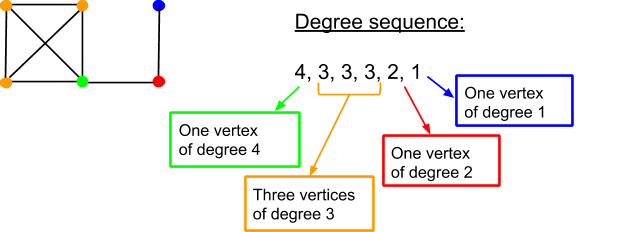
\includegraphics[width=6.5in]{degree-sequence.png}
  \paragraph{Connected} Two vertices are connected if there is a path between them. They are \textbf{disconnected} otherwise.
  \paragraph{Connected component} A maximal set of vertices that is connected, meaning no other vertex may be added to it without compromising its connectedness.
  \paragraph{Isolated vertex} A vertex not connected to any other vertex
  \paragraph{$k$-vertex-connected graph} A graph G is $k$-vertex-connected if the graph contains at least $k  _ 1$ vertices and remains connected after any $k -1$ vertices are removed from the graph. The \textbf{vertex connectivity} of a graph is the largest $k$ such that the graph is $k$-vertex-connected. The vertex connectivity of a graph $G$ is denoted $\kappa(G)$.
  \paragraph{$k$-edge-connected graph}An undirected graph G is k-edge-connected if it remains connected after any k - 1 edges are removed from the graph. The \textbf{edge connectivity} of a graph is the largest k such that the graph is k-edge-connected. The edge connectivity of a graph G is denoted $\lambda(G)$.
  \paragraph{Euler circuit} A circuit that contains every edge and every vertex
  \paragraph{Euler trail} An open trail that includes each edge
  \paragraph{Hamiltonian cycle} A cycle that includes every vertex in the graph
  \paragraph{Hamiltonian path} A path that includes every vertex in the graph
  \paragraph{Embedding} An assignment of the vertices in a graph to points in a 2-dimensional plane and an assignment of each edge to a continuous curve. An embedding is said to be a \textbf{planar embedding} if none of the edges cross. There is a \textbf{crossing} between two edges in an embedding if their curves intersect at a point that is not a common endpoint.
  \paragraph{Planar graph} A graph that has a planar embedding
  \paragraph{Exterior region} An infinite region outside of the space enclosed by a planar graph
  \paragraph{Complement of an embedding} The set of all points in the plane that are not a vertex or part of a curve corresponding to an edge
  \paragraph{Region} a set of points in the complement of an embedding that forms a maximal continuous set
  \paragraph{Graph coloring} Coloring can be used on a graph where there is a finite number of colors that can be assigned to vertices. No two adjacent vertices may be assigned the same color in order for the graph to have \textbf{valid coloring}. If $k$ is the number of colors used, then the graph is a $k$-coloring.
  \paragraph{Chromatic number} The smallest $k$ such that there is a valid $k$-coloring of the graph. If $G$ is a directed graph, then the chromatic number is denoted $X(G)$.
  \paragraph{Clique number} The largest $r$ such that $K_r$ is a subgraph of $G$, denoted $\omega(G)$
  \paragraph{Greedy coloring algorithm} An easy and natural method to color the vertices of a graph. Though it often uses a small number of colors, it has no guarantee that it will find the smallest number of colors possible. Steps follow:
  \begin{itemize}
    \item Number the set of possible colors. Assume that there is a very large supply of different colors, even though they might not all be used.
    \item Order the vertices in any arbitrary order.
    \item Consider each vertex v in order, and Assign v a color that is different from the color of v's neighbors that have already been assigned a color. When selecting a color for v, use the lowest numbered color possible.
  \end{itemize}
  The term ``greedy'' algorithm describes an algorithm that typically solves a problem one piece at a time.
  \pagebreak
  \section{Trees}
  \paragraph{Tree} An undirected graph that is connected and has no cycles
  \subparagraph{Free tree} A tree with no particular organization of the vertices and edges
  \subparagraph{Rooted tree} A tree with a vertex designated the \textbf{root} of the tree from where all other vertices stem
  \paragraph{Level} The level of a vertex is its distance from the root
  \paragraph{Height} The height of a tree is the highest level of any vertex
  \paragraph{Variable length codes} Binary strings of variable length that can be used to represent ASCII and Unicode characters
  \paragraph{Prefix} A string s is a prefix of another string t if all the characters in string s appear at the beginning of string t.
  \paragraph{Prefix code} Has the property that the code for one character con not be a prefix of the code for another character
  \paragraph{Internal vertex} A vertex in a tree that has a degree of at least two
  \paragraph{Forest} A graph that has no cycles and is not necessarily connected
  \paragraph{Tree traversal} A procedure to process the information stored in the vertices of a tree by systematically visiting each vertex
  \subparagraph{Pre-order traversal} Wherein a vertex is visited before its descendants
  \subparagraph{Post-order traversal} Wherein a vertex is visited after its descendants
  \paragraph{Spanning tree} A spanning tree of a connected graph G is a subgraph of G which contains all the vertices in G and is a tree
  \paragraph{Depth-First Search} Favors going deep into the graph and tends to produce trees with longer paths from the start vertex
  \paragraph{Breadth-First Search} visits vertices in the graph according to their proximity to the start vertex
  \paragraph{Spanning tree} A tree that specifies a subset of the edges that provides connectivity between every pair of vertices while minimizing the number of edges included. Spanning trees with n nodes has n-1 edges. A \textbf{minimum spanning tree (MST)} of a weighted graph is a spanning tree whose weight is no larger than any other spanning tree possible.
  \pagebreak
  \paragraph{Prim's algorithm}
  \begin{lstlisting}
Input: An undirected, connected, weighted graph G.
Output: T, a minimum spanning tree for G.

T := null.
Pick any vertex in G and add it to T.

For j = 1 to n-1
      Let C be the set of edges with one endpoint inside T and one endpoint outside T.
      Let e be a minimum weight edge in C.
      Add e to T.
      Add the endpoint of e not already in T to T.
End-for
  \end{lstlisting}
  \pagebreak
\section{Laws of Propositional Logic}
\paragraph{Idempotent laws}
\begin{align*}
 p \lor p \equiv p \\
 p \land p \equiv p
\end{align*}
\paragraph{Associative laws}
\begin{align*}
 (p \lor q) \lor r \equiv p \lor (q \lor r) \\
 (p \land q) \land r \equiv p \land (q \land r)
\end{align*}
\paragraph{Commutative laws}
\begin{align*}
 p \lor q \equiv q \lor p \\
 p \land q \equiv q \land p
\end{align*}
\paragraph{Distributive laws}
\begin{align*}
  p \lor (q \land r) \equiv (p \lor q) \land (p \lor r) \\
  p \land (q \lor r) \equiv (p \land q) \lor (p \land r)
\end{align*}
\paragraph{Identity laws}
\begin{align*}
 p \lor F \equiv p \\
 p \land T \equiv p
\end{align*}
\paragraph{Domination laws}
\begin{align*}
 p \land F \equiv F \\
 p \lor T \equiv T
\end{align*}
\paragraph{Double negation law}
\begin{align*}
 \lnot \lnot p \equiv p
\end{align*}
\paragraph{Complement laws}
\begin{align*}
 p \land \lnot p \equiv F \\
 p \lor \lnot p \equiv T \\
 \lnot T \equiv F \\
 \lnot F \equiv T
\end{align*}
\paragraph{De Morgan's laws}
\begin{align*}
  \lnot (p \lor q) \equiv \lnot p \land \lnot q \\
  \lnot (p \land q) \equiv \lnot p \lor \lnot q
\end{align*}
\paragraph{Absorption laws}
\begin{align*}
 p \lor (p \land q) \equiv p \\
 p \land (p \lor q) \equiv p
\end{align*}
\paragraph{Conditional identities}
\begin{align*}
  p \implies q \equiv \lnot p \lor q \\
  p \iff q \equiv (p \implies q) \land (q \implies p)
\end{align*}
\section{Rules of Inference}

\paragraph{Modus ponens}
  $\begin{array}{rl}
    & p \\
    & p \implies q \\
    \cline{2-2}
    &\therefore q
  \end{array}$
\paragraph{Modus tollens}
  $\begin{array}{rl}
    & \lnot q \\
    & p \implies q \\
    \cline{2-2}
    &\therefore \lnot p
  \end{array}$
\paragraph{Addition}
  $\begin{array}{rl}
    & p \\
    \cline{2-2}
    &\therefore p \lor q
  \end{array}$
\paragraph{Simplification}
  $\begin{array}{rl}
    & p \land q \\
    \cline{2-2}
    &\therefore p
  \end{array}$
\paragraph{Conjunction}
  $\begin{array}{rl}
    & p \\
    & q \\
    \cline{2-2}
    &\therefore p \land q
  \end{array}$
\paragraph{Hypothetical syllogism}
  $\begin{array}{rl}
    & p \implies q \\
    & q \implies r \\
    \cline{2-2}
    &\therefore p \implies r
  \end{array}$
\paragraph{Disjunctive syllogism}
  $\begin{array}{rl}
    & p \lor q \\
    & \lnot p \\
    \cline{2-2}
    &\therefore q
  \end{array}$
\paragraph{Resolution}
  $\begin{array}{rl}
    & p \lor q \\
    & \lnot p \lor r \\
    \cline{2-2}
    &\therefore q \lor r
  \end{array}$

  \paragraph{Universal instantiation}
  Let $c$ be an arbitrary or particular element:
  $\begin{array}{rl}
    & \forall x P(x) \\
    \cline {2-2}
    &\therefore P(c)
  \end{array}$
  \paragraph{Universal generalization}
  let $c$ be an arbitrary element: 
  $\begin{array}{rl}
    & P(c) \\
    \cline {2-2}
    &\therefore \forall x P(x)
  \end{array}$
  \paragraph{Existential instantiation}
  Let $c$ be a particular element: 
  $\begin{array}{rl}
    & \exists x P(x) \\
    \cline {2-2}
    &\therefore P(c)
  \end{array}$
  \paragraph{Existential generalization}
  let $c$ be an arbitrary or particular element: 
  $\begin{array}{rl}
    & P(c) \\
    \cline {2-2}
    &\therefore \exists x P(x)
  \end{array}$
  \pagebreak
  \section{Set Identities and Notable Sets}
\paragraph{Idempotent laws}
\begin{align*}
  A \cup A  =  A \\
  A \cap A  =  A
\end{align*}
\paragraph{Associative laws}
\begin{align*}
  (A \cup B) \cup C  =  A \cup (B \cup C) \\
  (A \cap B) \cap C  =  A \cap (B \cap C)
\end{align*}
\paragraph{Commutative laws}
\begin{align*}
  A \cup B  =  B \cup A \\
  A \cap B  =  B \cap A
\end{align*}
\paragraph{Distributive laws}
\begin{align*}
  A \cup (B \cap C)  =  (A \cup B) \cap (A \cup C) \\
  A \cap (B \cup C)  =  (A \cap B) \cup (A \cap C)
\end{align*}
\paragraph{Identity laws}
\begin{align*}
  A \cup \emptyset  =  A \\
A \cap \mathbb U  =  A
\end{align*}
\paragraph{Domination laws}
\begin{align*}
  A \cap \emptyset  =  \emptyset \\
  A \cup \mathbb U  =  \mathbb U
\end{align*}
\paragraph{Double complement law}
\begin{align*}
  \overline{\overline{A}}  =  A
\end{align*}
\paragraph{Complement laws}
\begin{align*}
A \cap \overline{A}  =  \emptyset \\
  A \cup \overline{A}  =  \mathbb U \\
\overline{\mathbb{U}}  =  \emptyset \\
  \overline{\emptyset}  =  \mathbb U
\end{align*}
\paragraph{De Morgan's laws}
\begin{align*}
\overline{A \cup B}  =  \overline{A} \cap \overline{B} \\
\overline{A \cap B}  =  \overline{A} \cup \overline{B}
\end{align*}
\paragraph{Absorption laws}
\begin{align*}
  A \cup (A \cap B)  =  A \\
  A \cap (A \cup B)  =  A
\end{align*}
\paragraph{Notable sets}
\begin{itemize}
  \item $\N$: set of natural numbers
  \item $\Z$: set of all integers
  \item $\Q$: set of rational numbers
  \item $\R$: set of real numbers
  \item $\U$: universal set
\end{itemize}
\paragraph{Properties of Sets in Functions}
\begin{itemize}
  \item $f: D \to T \implies |D| \leq |T|$ if $f$ is is injective
  \item $f: D \to T \implies |D| \geq |T|$ if $f$ is is surjective
  \item $f: D \to T \implies |D| = |T|$ if $f$ is is bijective
\end{itemize}

\pagebreak

\section{Laws of Boolean algebra and gate types}
\paragraph{Idempotent laws}
\begin{align*}
  x + x = x \\
  x \cdot x = x
\end{align*}
\paragraph{Associative laws}
\begin{align*}
  (x + y) + z = x + (y + z) \\
  (x  y)  z = x  (y  z)
\end{align*}
\paragraph{Commutative laws}
\begin{align*}
  x + y = y + x \\
  x  y = y  x
\end{align*}
\paragraph{Distributive laws}
\begin{align*}
  x + y  z = (x + y)  (x + z) \\
  x  (y + z) = x  y + x  z
\end{align*}
\paragraph{Identity laws}
\begin{align*}
  x + 0 = x \\
x \cdot 1 = x
\end{align*}
\paragraph{Domination laws}
\begin{align*}
  x \cdot 0 = 0 \\
  x + 1 = 1
\end{align*}
\paragraph{Double negation law}
\begin{align*}
  \overline{ \overline{ x}} = x
\end{align*}
\paragraph{Complement laws}
\begin{align*}
  x  \overline{ x }= 0 \\
  x + \overline{ x} = 1 \\
  \overline{ 1} = 0 \\
  \overline{ 0} = 1
\end{align*}
\paragraph{De Morgan's laws}
\begin{align*}
  \overline{ x + y} = \overline{ x}  \overline{ y} \\
  \overline{ x y} = \overline{ x} + \overline{ y}
\end{align*}
\paragraph{Absorption laws}
\begin{align*}
  x + (x  y) = x \\
  x  (x + y) = x
\end{align*}
\begin{figure}
  \caption{Gate types and circuit diagram symbols}
  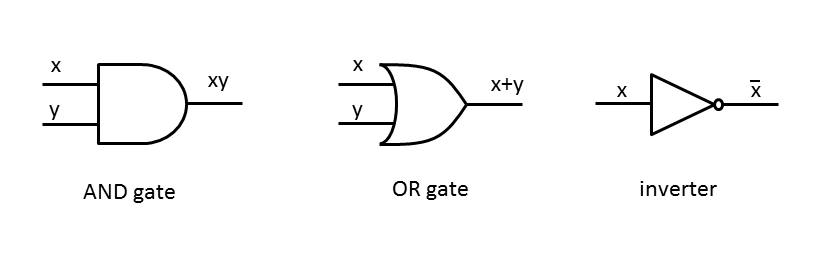
\includegraphics[width=6.5in]{3gates.png}
\end{figure}
\section{Rules for the asymptotic growth of a function that is the sum of other functions}
    
    \begin{equation*}
      f = O(h) \land g = O(h) \implies f + g = O(h)
    \end{equation*}
    
    \begin{equation*}
      f = \Omega (h) \lor g = \Omega (h) \implies f + g = \Omega (h)
    \end{equation*}
    
    \begin{equation*}
      f = O(g) \land c > 0 \implies c \cdot f = O (g)
    \end{equation*}
    
    \begin{equation*}
      f = \Omega (g) \land c > 0 \implies c \cdot f = \Omega(g)
    \end{equation*}
    
    \begin{equation*}
      f = O(g) \land g = O(h) \implies f = O(h)
    \end{equation*}
    
    \begin{equation*}
      f = \Omega (g) \land g = \Omega(h) \implies f = \Omega(h)
    \end{equation*}
\pagebreak

\section{Components of a Turing machine}
\begin{itemize}
  \item $Q$ Finite set of states
  \item $\Gamma$ Finite set of tape symbols
  \item $\Sigma \subset \Gamma$ A subset of the tape symbols are input symbols
  \item $q_0 \in Q$ The start state
  \item $q_{acc} \in Q$ The accept state
  \item $q_{rej} \in Q$ The reject state
  \item $\delta: (Q - \{q_{acc}, q_{rej}\}) \times \Gamma \to Q \times \Gamma \times \{L, R\}$ Transition function
\end{itemize}

\section{Fundamental connections for polynomial functions}
For a polynomial $f$ and a real number $k$,
\paragraph{Root} $x = k$ is a root, or solution, of the equation $f(x) = 0$
\paragraph{Zero} $k$ is a zero of function $f$ when $f(x) = 0$
\paragraph{Linear factor} $x - k$ is a linear factor of $f(x)$
\paragraph{Multiplicity} When a linear factor occurs multiple times in the factorization of a polynomial, that gives the related zero multiplicity. Ex: in the polynomial $f(x) = (x-1)(x-4)^2$, the number 4 is a zero of multiplicity 2.
\pagebreak
\begin{figure}
  \caption{Common graphs in graph theory}
  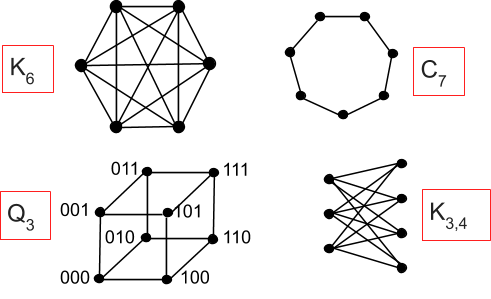
\includegraphics[width=6.5in]{common-graphs.png}
\end{figure}
\begin{itemize}
  \item $K_n$ is called the \textbf{complete graph} on $n$ vertices. $K_n$ is sometimes called a \textbf{clique} of size $n$ or an $n$-clique.
  \item $C_n$ is called a cycle on $n$ vertices.
  \item $Q_n$ is called an $n$-dimensional hypercube.
\end{itemize}
\pagebreak
\section{Theorems}
\paragraph{The Graph Power Theorem}
  Let $G$ be a directed graph. Let $u$ and $v$ be any two vertices in $G$. There is an edge from $u$ to $v$ in $G^k$ if and only if there is a walk of length $k$ from $u$ to $v$ in $G$.
\paragraph{Relationship between the powers of a graph and the powers of its adjacency matrix}
Let G be a directed graph with n vertices and let A be the adjacency matrix for G. Then for any $k \geq 1$, $A^k$ is the adjacency matrix of $G^k$, where Boolean addition and multiplication are used to compute $A^k$.
\paragraph{Addition and graph union}
Let G and H be two directed graphs with the same vertex set. Let A be the adjacency matrix for G and B the adjacency matrix for H. Then the adjacency matrix for $G \cup H$ is A + B, where Boolean addition used on the entries of matrices A and B. 
\paragraph{Directed acyclic graphs and strict orders}
Let $G$ be a directed graph. $G$ has no positive length cycles if and only if $G^+$ is a strict order.
\paragraph{Structure of equivalence relations}
Consider an equivalence relation on a set $A$. Let $x,y \in A$:
\begin{itemize}
  \item $x \sim y \implies [x] = [y]$
  \item $\lnot x \sim y \implies [x] \cap [y] = \emptyset$
\end{itemize}
\paragraph{Equivalence relations define a partition}
Consider an equivalence relation over a set A. The set of all distinct equivalence classes defines a partition of A. The term "distinct" means that if there are two equal equivalence classes [a] = [b], the set [a] is only included once.
\paragraph{Explicit formula for a sequence defined by a summation}
for every positive integer $n$, 
\begin{equation*}
  \sum_{j = 1}^{n} j = \frac{n(n + 1)}{2} 
\end{equation*}
\paragraph{Explicit formula for a sequence defined by a recurrence relation}
Define the sequence $\{g_n\}$ as:
\begin{itemize}
  \item $g_0 = 1$
  \item $g_n = 3 \cdot g_{n-1} + 2n \land n \geq 1$
\end{itemize}
Then for any $n \geq 0$, 
\begin{equation*}
  g_n = \frac{5}{2} \cdot 3^n - n - \frac{3}{2}
\end{equation*}
\paragraph{Explicit formula for a sequence defined by a recurrence relation}
Define the sequence $\{h_n\}$ as:
\begin{itemize}
  \item $h_0 = 7$
  \item $h_n = (h_{n-1})^3 \land n \geq 1$
\end{itemize}
Then for any $n \geq 0$, 
\begin{equation*}
  h_n = 7^{(3^n)}
\end{equation*}
\paragraph{Number of vertices in a perfect binary tree}
Let $T$ be a perfect binary tree. Then the number of vertices in $T$ is $2^k - 1$ for some positive integer $k$. ($k$ is the number of times the recursive rule of a binary tree has been applied to the initial vertex
\paragraph{The form of particular solutions to certain linear non-homogeneous recurrence relations}
Let $F(n)$ be a function that includes all the non-homogeneous terms. Suppose the sequence $\{f_n\}$ is described by the linear non-homogeneous recurrence relation
\begin{equation*}
  f_n = \sum_{k=1}^{d} (c_k f_{n-k}) + F(n)
\end{equation*}
and suppose that the function $F(n)$ has the form $F(n) = p(n)s^n$, where $p(n)$ is a polynomial of degree $t$ and $s$ is a constant.
\begin{itemize}
  \item If $s$ is not a root of the characteristic equation for the associated homogeneous recurrence relation, then there is a particular solution of the form
    \begin{equation*}
      f_n = \sum_{k=0}^{t} (d_{t-k} n^{t-k}) s^n
    \end{equation*}
  \item If $s$ is a root of the characteristic equation for the associated homogeneous recurrence relation of multiplicity $m$, then there is a particular solution of the form 
    \begin{equation*}
      f_n = n^m \sum_{k=0}^{t} (d_{t-k} n^{t-k}) s^n
    \end{equation*}
\end{itemize}
\paragraph{The Master Theorem for determining algorithmic complexity of divide-and-conquer recurrence relations}
Let the function $T$ represent the time complexity of a divide-and-conquer algorithm. On a call to the algorithm with input of size $n$, $\Theta(n^d)$ operations are performed outside the recursive calls. In addition, there are $a$ recursive calls made on inputs of size $n/b$, where $b$ is the number of sub-lists. This yields the form
\begin{equation*}
  T(n) = aT(n/b)+\Theta(n^d)
\end{equation*}
For constants $a > 0$, $b > 1$, and $d \geq 0$
\begin{itemize}
  \item $(a/b^d) < 1 \implies T(n) = \Theta(n^d)$
  \item $(a/b^d) = 1 \implies T(n) = \Theta(n^d \log n)$
  \item $(a/b^d) > 1 \implies T(n) = \Theta(n^{\log_b a})$
\end{itemize}
\paragraph{Baye's Theorem}
Suppose that $F$ and $X$ are events from a common sample space and $p(F) \neq 0 \land p(X) \neq 0$. Then
\begin{align*}
  p(F|X) &= \frac{P(F \cap X)}{p(F)}\\
    &= \frac{p(X|F) p(F)}{P(F)}\\
    &= \frac{p(X|F) p(F)}{p(X|F) p(F) + p(X|\overline{F}) p(\overline{F})}
\end{align*}
\paragraph{An alternative way to calculate the expectation of a random variable}
If $X$ is a random variable defined over an experiment with sample space $S$,
\begin{equation*}
  E[x] = \sum_{r \in X(S)}^{} r \cdot p(X = r)
\end{equation*}
Where $X(S)$ is the range of the function $X$
\paragraph{linearity of expectations}
If $X$ and $Y$ are two random variables defined on the same sample space $S$, and $c$ is a real number,
\begin{align*}
  E[X + Y] &= E[X] + E[Y]\\
  E[cX] &= cE[X]
\end{align*}
\paragraph{Bernoulli trial probabilities}
The probability of exactly $k$ successes in a sequence of $n$ independent Bernoulli trials, with probability of success $p$ and probability of failure $q = 1-p$ is
\begin{equation*}
  \binom{n}{k} p^k q^{n-k}
\end{equation*}
\paragraph{Number of edges and total degree}
Let $G = (V, E)$ be an undirected graph. Then twice the number of edges is equal to the total degree:
\begin{equation*}
  \sum_{v \in V}^{} deg(v) = 2 \cdot |E|
\end{equation*}
\paragraph{Vertex degree preserved under isomorphism}
Consider two graphs, $G$ and $G'$. Let $f$ be an isomorphism from $G$ to $G'$. For each vertex $v$ in $G$, the degree of vertex $v$ in $G$ is equal to the degree of vertex $f(v)$ in $G$.
\paragraph{Upper bound for vertex and edge connectivity}
Let $G$ be an undirected graph. Denote the minimum degree of any vertex in $G$ by $\delta(G)$. Then the two inequalities hold true:
\begin{equation*}
  \kappa(G) \leq \delta(G)
\end{equation*}
\begin{equation*}
  \lambda(G) \leq \delta(G)
\end{equation*}
\paragraph{Required conditions for an Euler circuit in a graph}
If an undirected graph $G$ has an Euler circuit, then $G$ is connected and every vertex in $G$ has an even degree.
\paragraph{Characterizations of graphs that have an Euler trail} 
An undirected graph $G$ has an Euler trail if and only if $G$ is connected and has exactly two vertices with odd degree.
\paragraph{Euler's Identity}
Consider a planar embedding of a connected graph $G$. Let $n$ be the number of vertices in $G$, $m$ the number of edges, and $r$ the number of regions in the embedding. Then,
\begin{equation*}
  n = m + r = 2
\end{equation*}
\paragraph{Number of edges in a planar graph}
Let $G$ be a connected planar graph. Let $n$ be the number of vertices in $G$ and $m$ the number of edges. If $n \geq 3$, then
\begin{equation*}
  m \leq 3n - 6
\end{equation*}
\paragraph{Relationship between the clique number and chromatic number}
If $G$ is an undirected graph, then $\omega(G) \leq X(G)$.
\paragraph{Upper bound for $X(G)$}
Let G be an indirected graph. Let $\Delta(G)$ be the maximum degree of any vertex in $G$. Then,
\begin{equation*}
  X(G) \leq \Delta(G) + 1
\end{equation*}
\end{document}
